\section{Introduction}\label{sec:intro}
An important question plaguing machine learning is \cite{BenAli-1,Lecun,BenAli-2,Aliresponse,Mickens}:\\
{\centerline{\textbf{\emph{Is Deep Learning Alchemy?}}}}\\
At the centre of this question is the lack of \emph{pedagogical nuggets} of ``simple theorems, simple experiments" \cite{Aliresponse} that explain in an interpretable way the success of \emph{practical}\footnote{Off-the-shelf deep networks trained using stochastic gradient descent starting from randomised initialisation.} deep neural networks (DNNs). The goal of this paper is to propose one such pedagogical nugget to explain (i) training/generalisation, (ii) roles of activations, weights, depth, width, skip connections and convolutions with pooling for DNNs with rectified linear units (ReLUs). We exploit the special \emph{gating property} of ReLU, i.e., each ReLU is also a gate which either blocks (multiplies by $0$) or allows its pre-activation input (multiplies by $1$). 
%By \emph{practical} DNNs, we mean standard off-the-shelf DNN architectures trained using stochastic gradient descent starting from randomised initialisation, and we choose to exclude pure function approximation results \citet{depth1,depth2}.

Recent works by \citet{arora2019exact, ntk,cao2019generalization} have shown that training an infinite width DNN is equivalent to a kernel method with the so called limiting \emph{neural tangent kernel} (NTK) matrix. \citet{arora2019exact} showed that the limiting Convolutional NTK (CNTK) corresponding to a convolutional neural network (CNN) beats other pure kernel based methods. However, the CNN still outperforms the CNTK by $5-6\%$. So, the NTK does not fully explain the success of finite width DNNs. Also, it is not known why depth and pooling helps both the CNTK as well the CNN \cite{arora2019exact}.

Recently, \citet{npk} developed a dual view for DNNs with ReLUs to study the role of gates. In the dual view, the computations are broken down \emph{path-by-path} as opposed to the primal view where the computations proceed \emph{layer-by-layer}. This provides a \emph{sub-network} based interpretation for DNNs: each input has a corresponding \emph{active sub-network} comprising of the gates that are \emph{on} and weights through such gates, that produces the output. They also showed via theory and experiments that most information is stored in the gates (\emph{on/off} states of ReLU). The highlights are presented in the bulleted points below.

$\bullet$ \emph{Theory:} In the limit of infinite width, weights initialised statistically independent of arbitrary gates, the NTK is equal (up to a scaling constant) to the \emph{neural path kernel} (NPK), a kernel solely dependent on the information in the gates. %\emph{Hadamard} product of Gram matrix and a correlation matrix that measures the amount overlap in the active sub-networkss for the various pairs input examples.

$\bullet$ \emph{Experiments:} While the NPK characterises the gates theoretically, a deep gated network (DGN) was proposed to experimentally characterise the information in the gates of finite width DNNs. This is a significant deviation from design and analysis based on kernels associated with infinite width DNNs at randomised initialisation \cite{arora2019exact,fcgp,convgp}. In a DGN, the gates and the weights are held in separate networks as opposed to a DNN which holds them in the same network (see \Cref{fig:dgn}).  It was shown that (i)  \emph{most information is in the gates:} by just using the gates of a pre-trained DNN (by letting it to be the gating network), the weight network can be trained to match the test performance (within $1\%$ ) of the DNN, and (ii) \emph{learning of gates} during training explains the difference between finite width CNN and the infinite width CNTK.  %Instead of devising a pure kernel method based on the NPK, a deep gated network (DGN) was proposed. 
\FloatBarrier
\begin{figure}[h]
\centering
%\resizebox{\columnwidth}{!}{
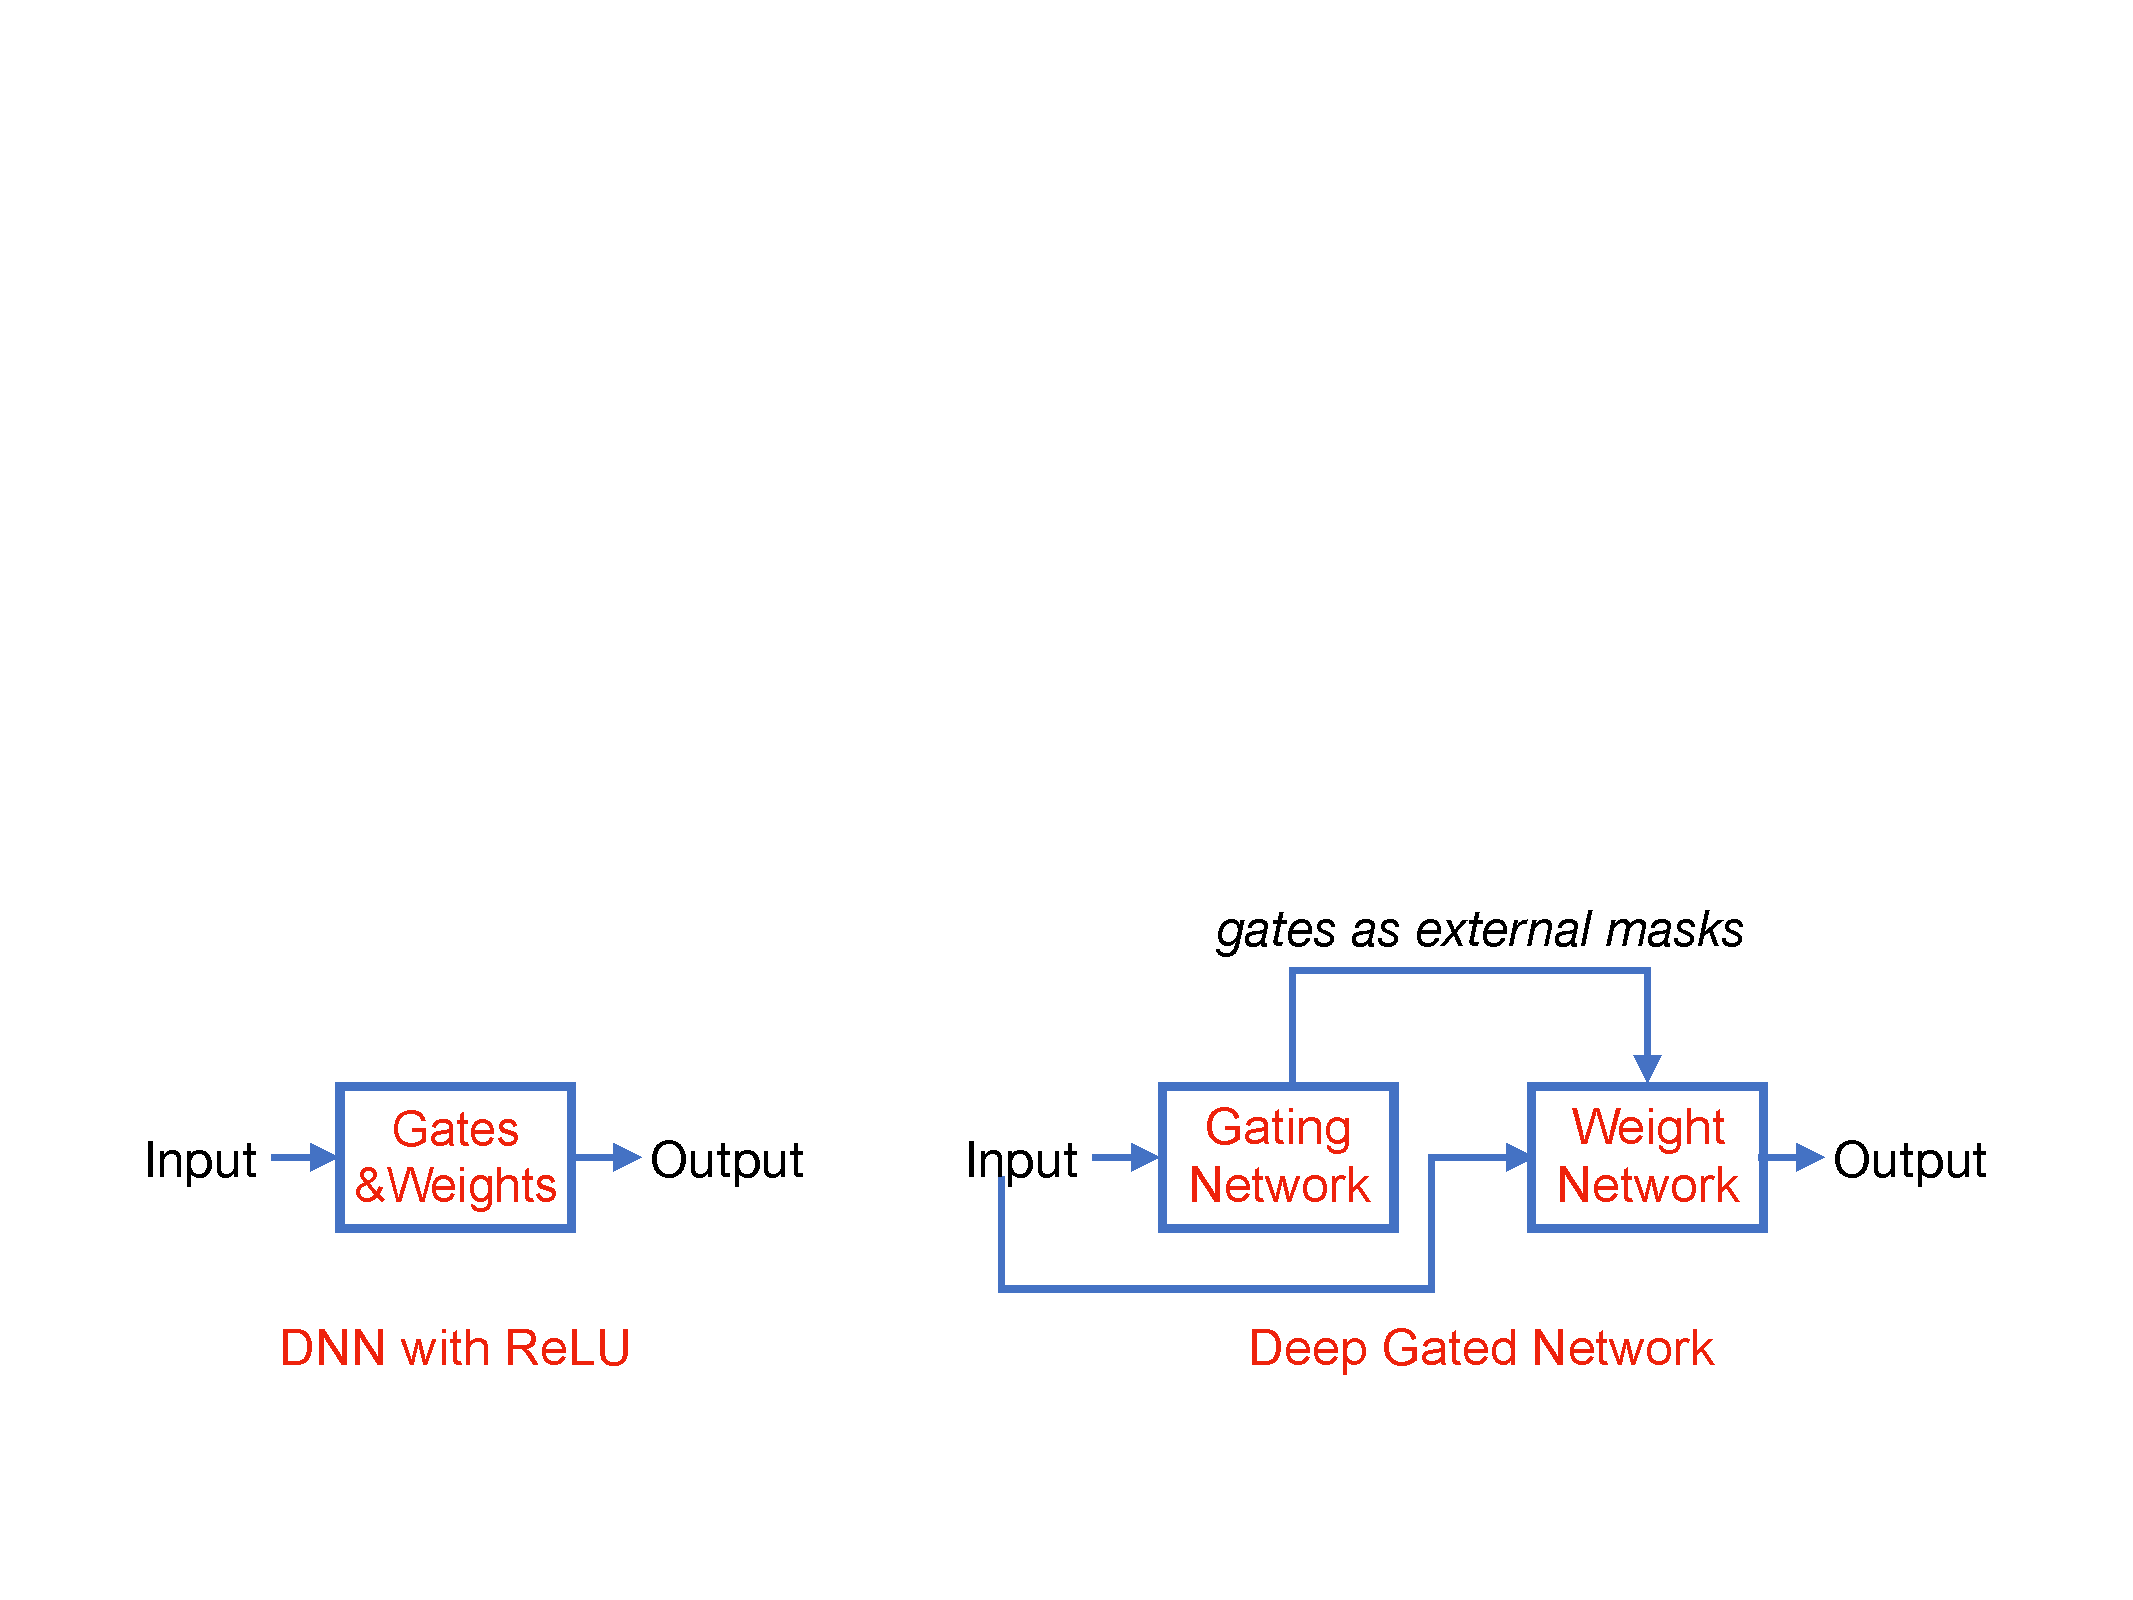
\includegraphics[scale=0.22]{figs/dnn-dgn.pdf}
%}
\caption{\small{DNN vs DGN. DNN-DGN $<1\%$.}}
\label{fig:dgn}
\end{figure}
\begin{comment}
 The \emph{alchemy} question can further be broken down into sub-questions/issues/gaps as listed below. \\
1. \emph{Training:} Despite a \emph{non-convex} loss surface, why is it possible for stochastic gradient descent (SGD) (and its variants) to achieve zero training error in standard deep neural networks (DNNs)?\\
2. \emph{Generalisation:} Standard DNNs are \emph{over-parameterised}, yet, when trained on data with true labels we observe good test performance \citet{ben}.\\
3. \emph{Functionality:} The roles of the basic parts/variables namely weights, activation, depth and width have not been clearly understood. The standard understanding is that, in each layer, weights perform of a linear operation, the activations perform a non-linear operation, and width determines dimensions of the hidden features (i.e., outputs of the hidden layers).  Approximation theory based results \citet{depth1,depth2} show that deeper models can approximate more complicated target functions better than shallow models. However,  \emph{practical} DNNs are trained/tested on standard datasets (such as MNIST and CIFAR-10) using SGD (and variants) starting from randomly initialised weights. Since not all representable functions can also be reached in practical DNNs the applicability of approximation results to practical DNNs is questionable. Further, convolutions with pooling and skip connections are also required for success of practical DNNs. \\
4. \emph{Uninterpretablity} of features learnt in hidden layers.\\ 
 We propose a \emph{pedagogical nugget} of ``simple theorems, and simple experiments" \citet{Aliresponse} to explain (i) training/generalisation, (ii) roles of activations, weights, depth, width, skip connections and convolutions with pooling for DNNs with rectified linear units (ReLUs). Our work is based on two prior works by (i) \citet{npk} on \emph{duality} and, (ii) by \citet{arora2019exact, ntk,cao2019generalization} on the  \emph{neural tangent kernel} (NTK).
The \emph{alchemy} question can further be broken down into sub-questions/issues/gaps as listed below. \\
1. \emph{Training:} Despite a \emph{non-convex} loss surface, why is it possible for stochastic gradient descent (SGD) (and its variants) to achieve zero training error in standard deep neural networks (DNNs)?\\
2. \emph{Generalisation:} Standard DNNs are \emph{over-parameterised}, yet, when trained on data with true labels we observe good test performance \citet{ben}.\\
3. \emph{Functionality:} The roles of the basic parts/variables namely weights, activation, depth and width have not been clearly understood. The standard understanding is that, in each layer, weights perform of a linear operation, the activations perform a non-linear operation, and width determines dimensions of the hidden features (i.e., outputs of the hidden layers).  Approximation theory based results \citet{depth1,depth2} show that deeper models can approximate more complicated target functions better than shallow models. However,  \emph{practical} DNNs are trained/tested on standard datasets (such as MNIST and CIFAR-10) using SGD (and variants) starting from randomly initialised weights. Since not all representable functions can also be reached in practical DNNs the applicability of approximation results to practical DNNs is questionable. Further, convolutions with pooling and skip connections are also required for success of practical DNNs. \\
4. \emph{Uninterpretablity} of features learnt in hidden layers.\\ 
\textbf{Our Work:} We propose a \emph{pedagogical nugget} of ``simple theorems, and simple experiments" \citet{Aliresponse} to explain (i) training/generalisation, (ii) roles of activations, weights, depth, width, skip connections and convolutions with pooling for DNNs with rectified linear units (ReLUs). \\
\textbf{Message:} We show that a DNN (with ReLU) can be simplified into \emph{atomic} units. Just as a single perceptron is characterised by a hyperplane, a DNN (with ReLU) being a multi-layered-perceptron is \emph{almost completely} characterised by the collection of hyperplanes (associated with the ReLUs that form the DNN).

The \emph{alchemy} question can further be broken down into sub-questions/issues/gaps as listed below. 

1. \emph{Training:} Despite a \emph{non-convex} loss surface, why is it possible for stochastic gradient descent (SGD) (and its variants) to achieve zero training error in standard deep neural networks (DNNs)?

2. \emph{Generalisation:} Standard DNNs are \emph{over-parameterised}, yet, when trained on data with true labels we observe good test performance. Does understanding deep learning require rethinking generalisation? \citet{ben}

%3. \emph{Depth:} Approximation results show that more depth is better \citet{depth1,depth2}, i.e., deeper models can approximate more complicated target functions better than shallow models. Yet, when training on standard datasets, increasing the depth beyond a point adversely affects both training and test performance \citet{resnets}. This situation can be remedied by using \emph{skip connections} giving rise to residual neural networks. However, why increasing depth beyond a point hurts standard DNNs is still not understood satisfactorily. 

%4. \emph{Depth vs Width:} Wider models \citet{wide1,wide2,wide3} have also been quite successful. While increasing either depth or width causes an increase in the number of model parameters, the trade-off between width and depth is not clearly understood.

4. \emph{Functionality:} The roles of the basic parts/variables namely weights, activation, depth and width have not been clearly understood. For instance, approximation results show that more depth is better \citet{depth1,depth2}, yet, when training on standard datasets, increasing the depth beyond a point adversely affects both training and test performance \citet{resnets}. Also, wider models \citet{wide1,wide2,wide3} have also been quite successful. While increasing either depth or width causes an increase in the number of model parameters, the roles of  width and depth in practical DNNs is not clearly understood.

5. \emph{Uninterpretablity of Learnt Representation:} The commonly held view of feature learning is that lower level features are learnt in the initial layers and as one proceeds in depth more sophisticated features are learnt in the higher levels and the final layer learns a linear model in the features given by the output of the penultimate layer. However, there is no straightforward way to interpret the features learnt in the hidden layers.

\end{comment}
\begin{comment}
\subsection{Methodology: Neural Tangent Kernel and Duality}
Our work is based on two prior works namely (i) \emph{duality} and (ii) \emph{neural tangent kernel} (NTK) (see also \Cref{fig:related}).\\
\textbf{Neural Tangent Kernel:} One of the approaches to understand the training and generalisation of a DNN is to study kernels associated with the DNN. Two important kernels associated with a DNN are its \emph{Conjugate Kernel (CK)/ Gaussian Process Kernel (GPK)} and the so called \emph{Neural Tangent Kernel (NTK)} . The CK is the Gram matrix of the features obtained at the penultimate layer output of the DNN. The NTK is Gram matrix of the Jacobian output of the DNN with respect to its weights. As width approaches to infinity, both the CK and the NTK converge to (their corresponding) limiting deterministic matrices. It has been shown that training the last layer of the infinite width DNN (known as \emph{lazy training}) is equivalent to a kernel method with the limiting CK and training all the layers of an infinite width DNN (known as \emph{full training}) is equivalent to a kernel method with the limiting NTK. Thus training and generalisation of infinite width DNNs boils down to the properties of the limiting deterministic kernel matrix. On CIFAR-10, the test accuracy of CK, NTK and standard DNN (all of three of them use convolution layers) is as follows:
\resizebox{\columnwidth}{!}{
\begin{tabular}{ccc}
CK & NTK & Standard\\
\citet{convgp} & \citet{arora2019exact} &  DNN\\
$\approx 67\%$&$\approx 77\%$&$80\%$ and above
\end{tabular}
}
The NTK performs better than the CK as well as other prior pure kernel based methods \citet{arora2019exact}. However, standard finite width DNN (with convolutional layers) still outperforms its infinite width NTK counterpart. As a result, NTK was not fully adequate to explain DNNs.
\FloatBarrier
\begin{figure}[h]
\centering
\resizebox{\columnwidth}{!}{
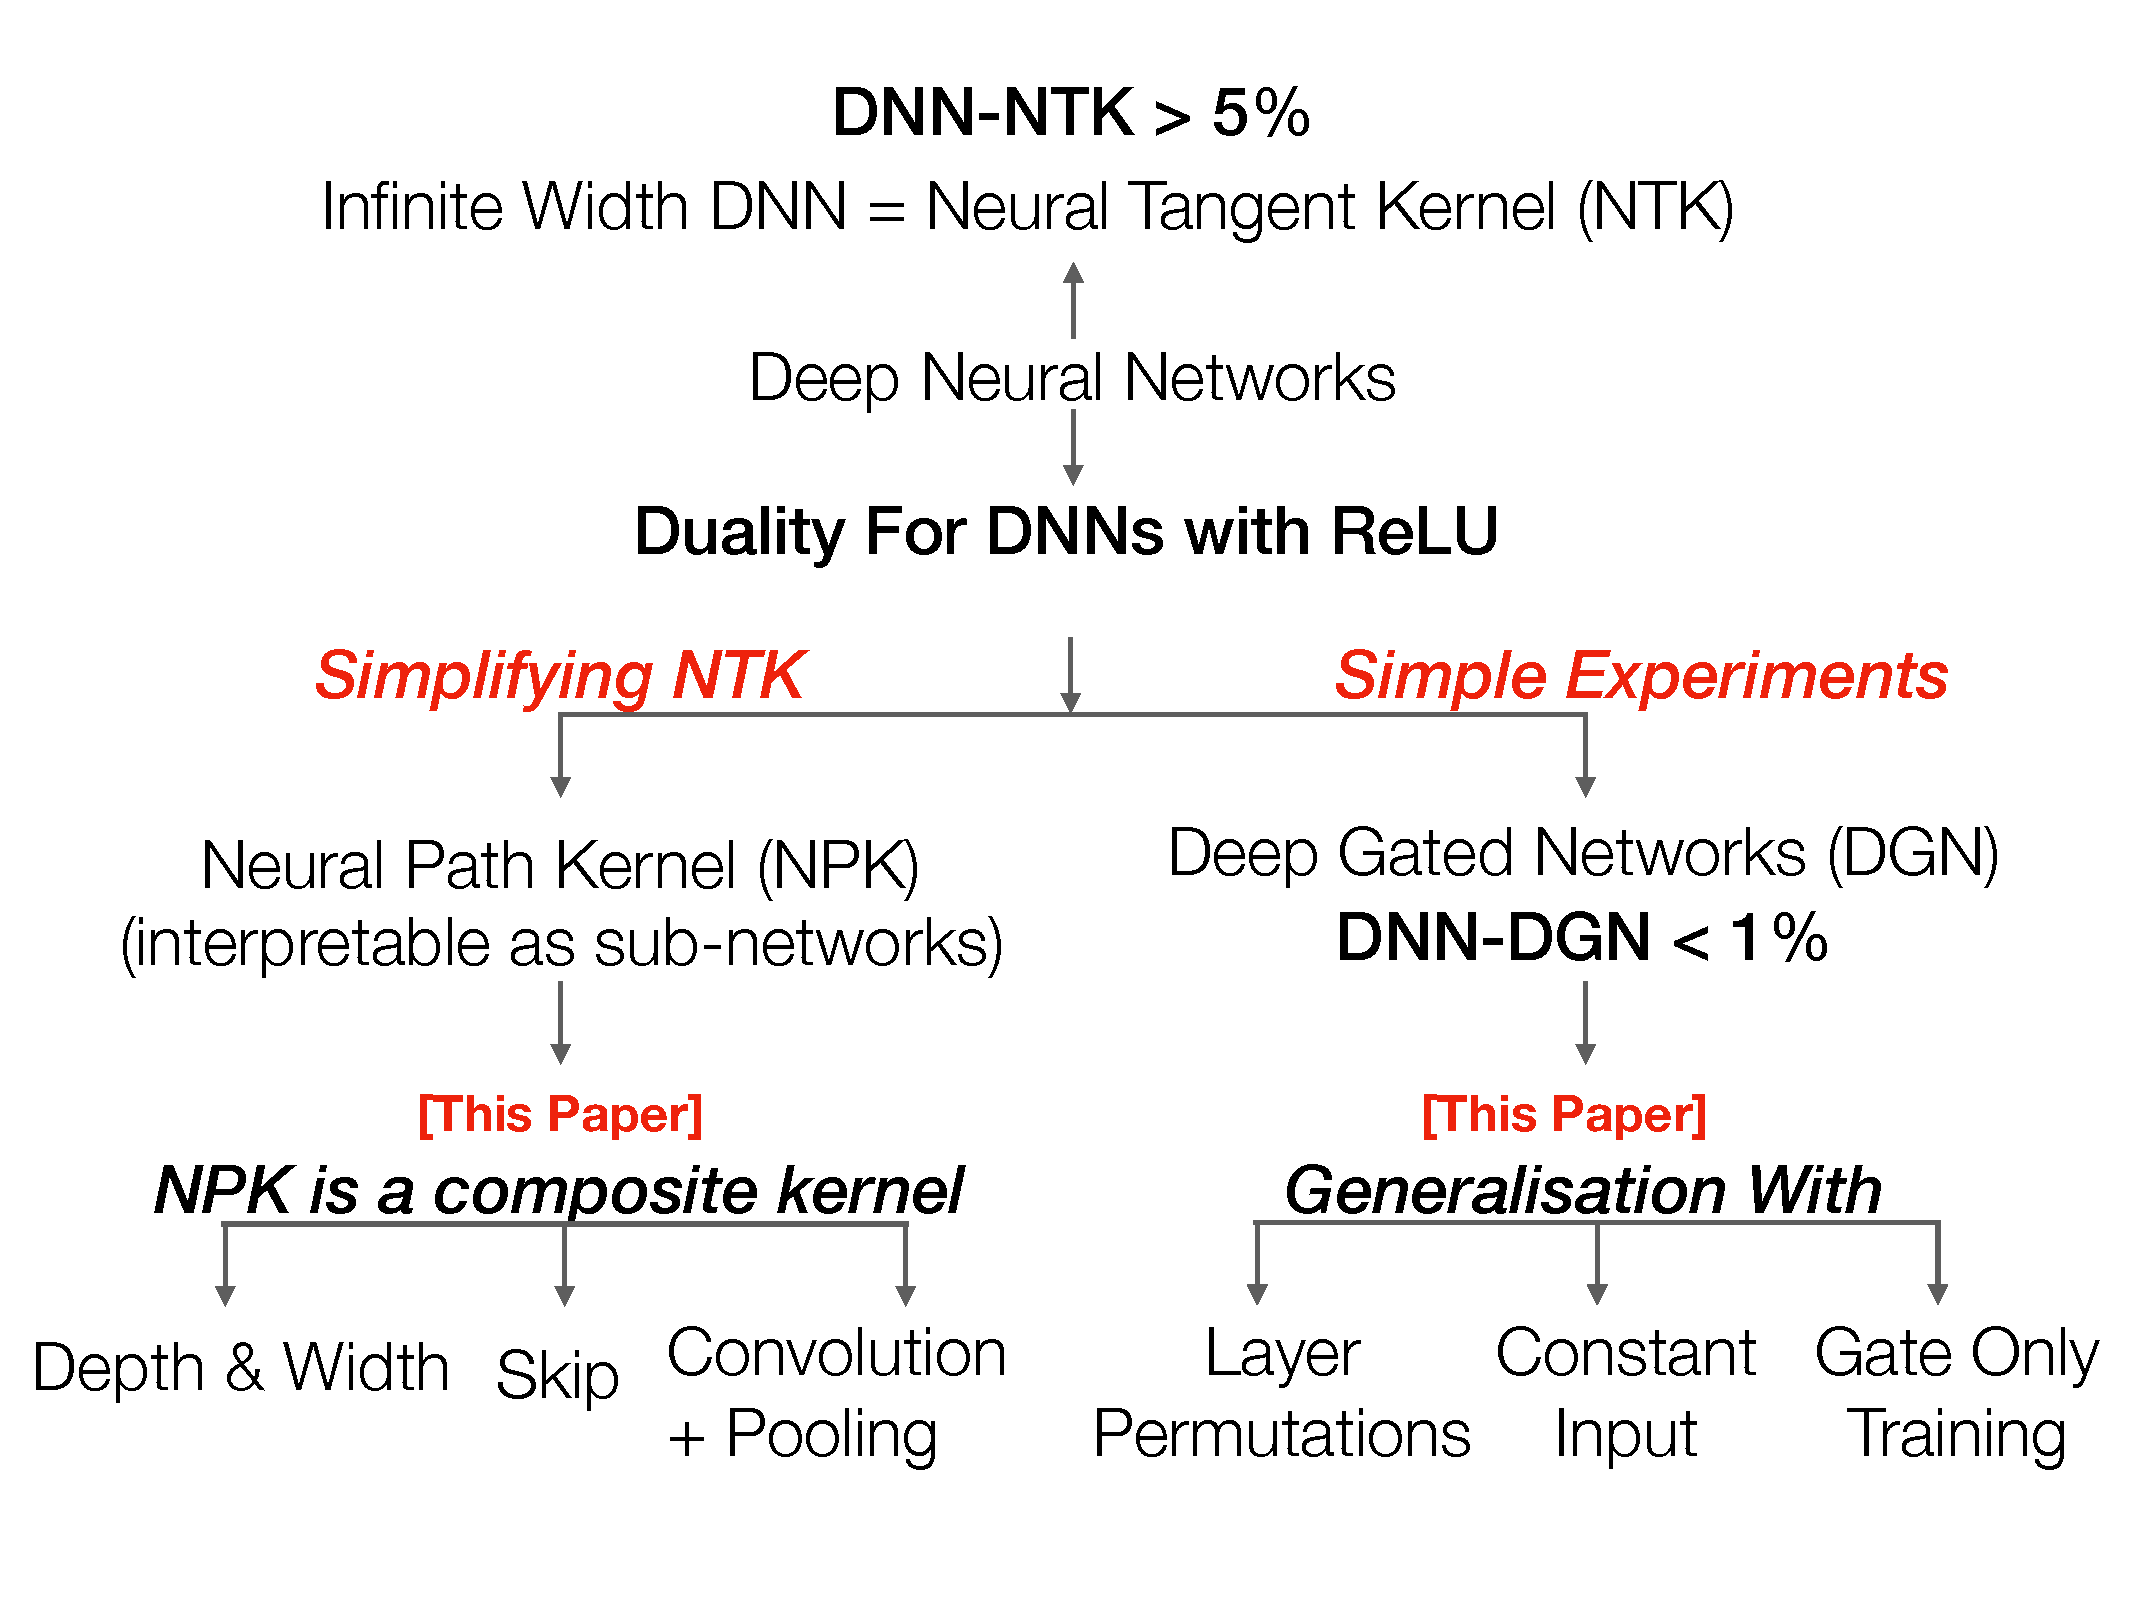
\includegraphics[scale=0.25]{figs/related.pdf}
}
\caption{This paper in relation to (i) NTK, (ii) Duality.}
\label{fig:related}
\end{figure}

\textbf{Duality (in DNNs with ReLU)}  enables the output of a DNN to be expressed as summation of individual paths. Duality is possible due to the special gating property of ReLU, i.e., each ReLU is also a gate which either blocks or allows its pre-activation input. Using duality \citet{npk} devised a setup called the deep gated network (DGN) and also simplified the NTK. 

\textbf{DGN (simple experiments with gates) :} Here, the gates and the weights are held in separate networks as opposed to a DNN in which gates and weights are in the same network (see \Cref{fig:dgn}). The speciality of the DGN is that it can handle arbitrary gates, i.e., the gating network weights can be arbitrary and not necessarily random. This enables one to compare random gates (at randomised initialisation) and learnt gates (at end of training). Using the DNG, \citet{npk} showed the following.
\FloatBarrier
\begin{figure}[h]
\centering
\resizebox{\columnwidth}{!}{
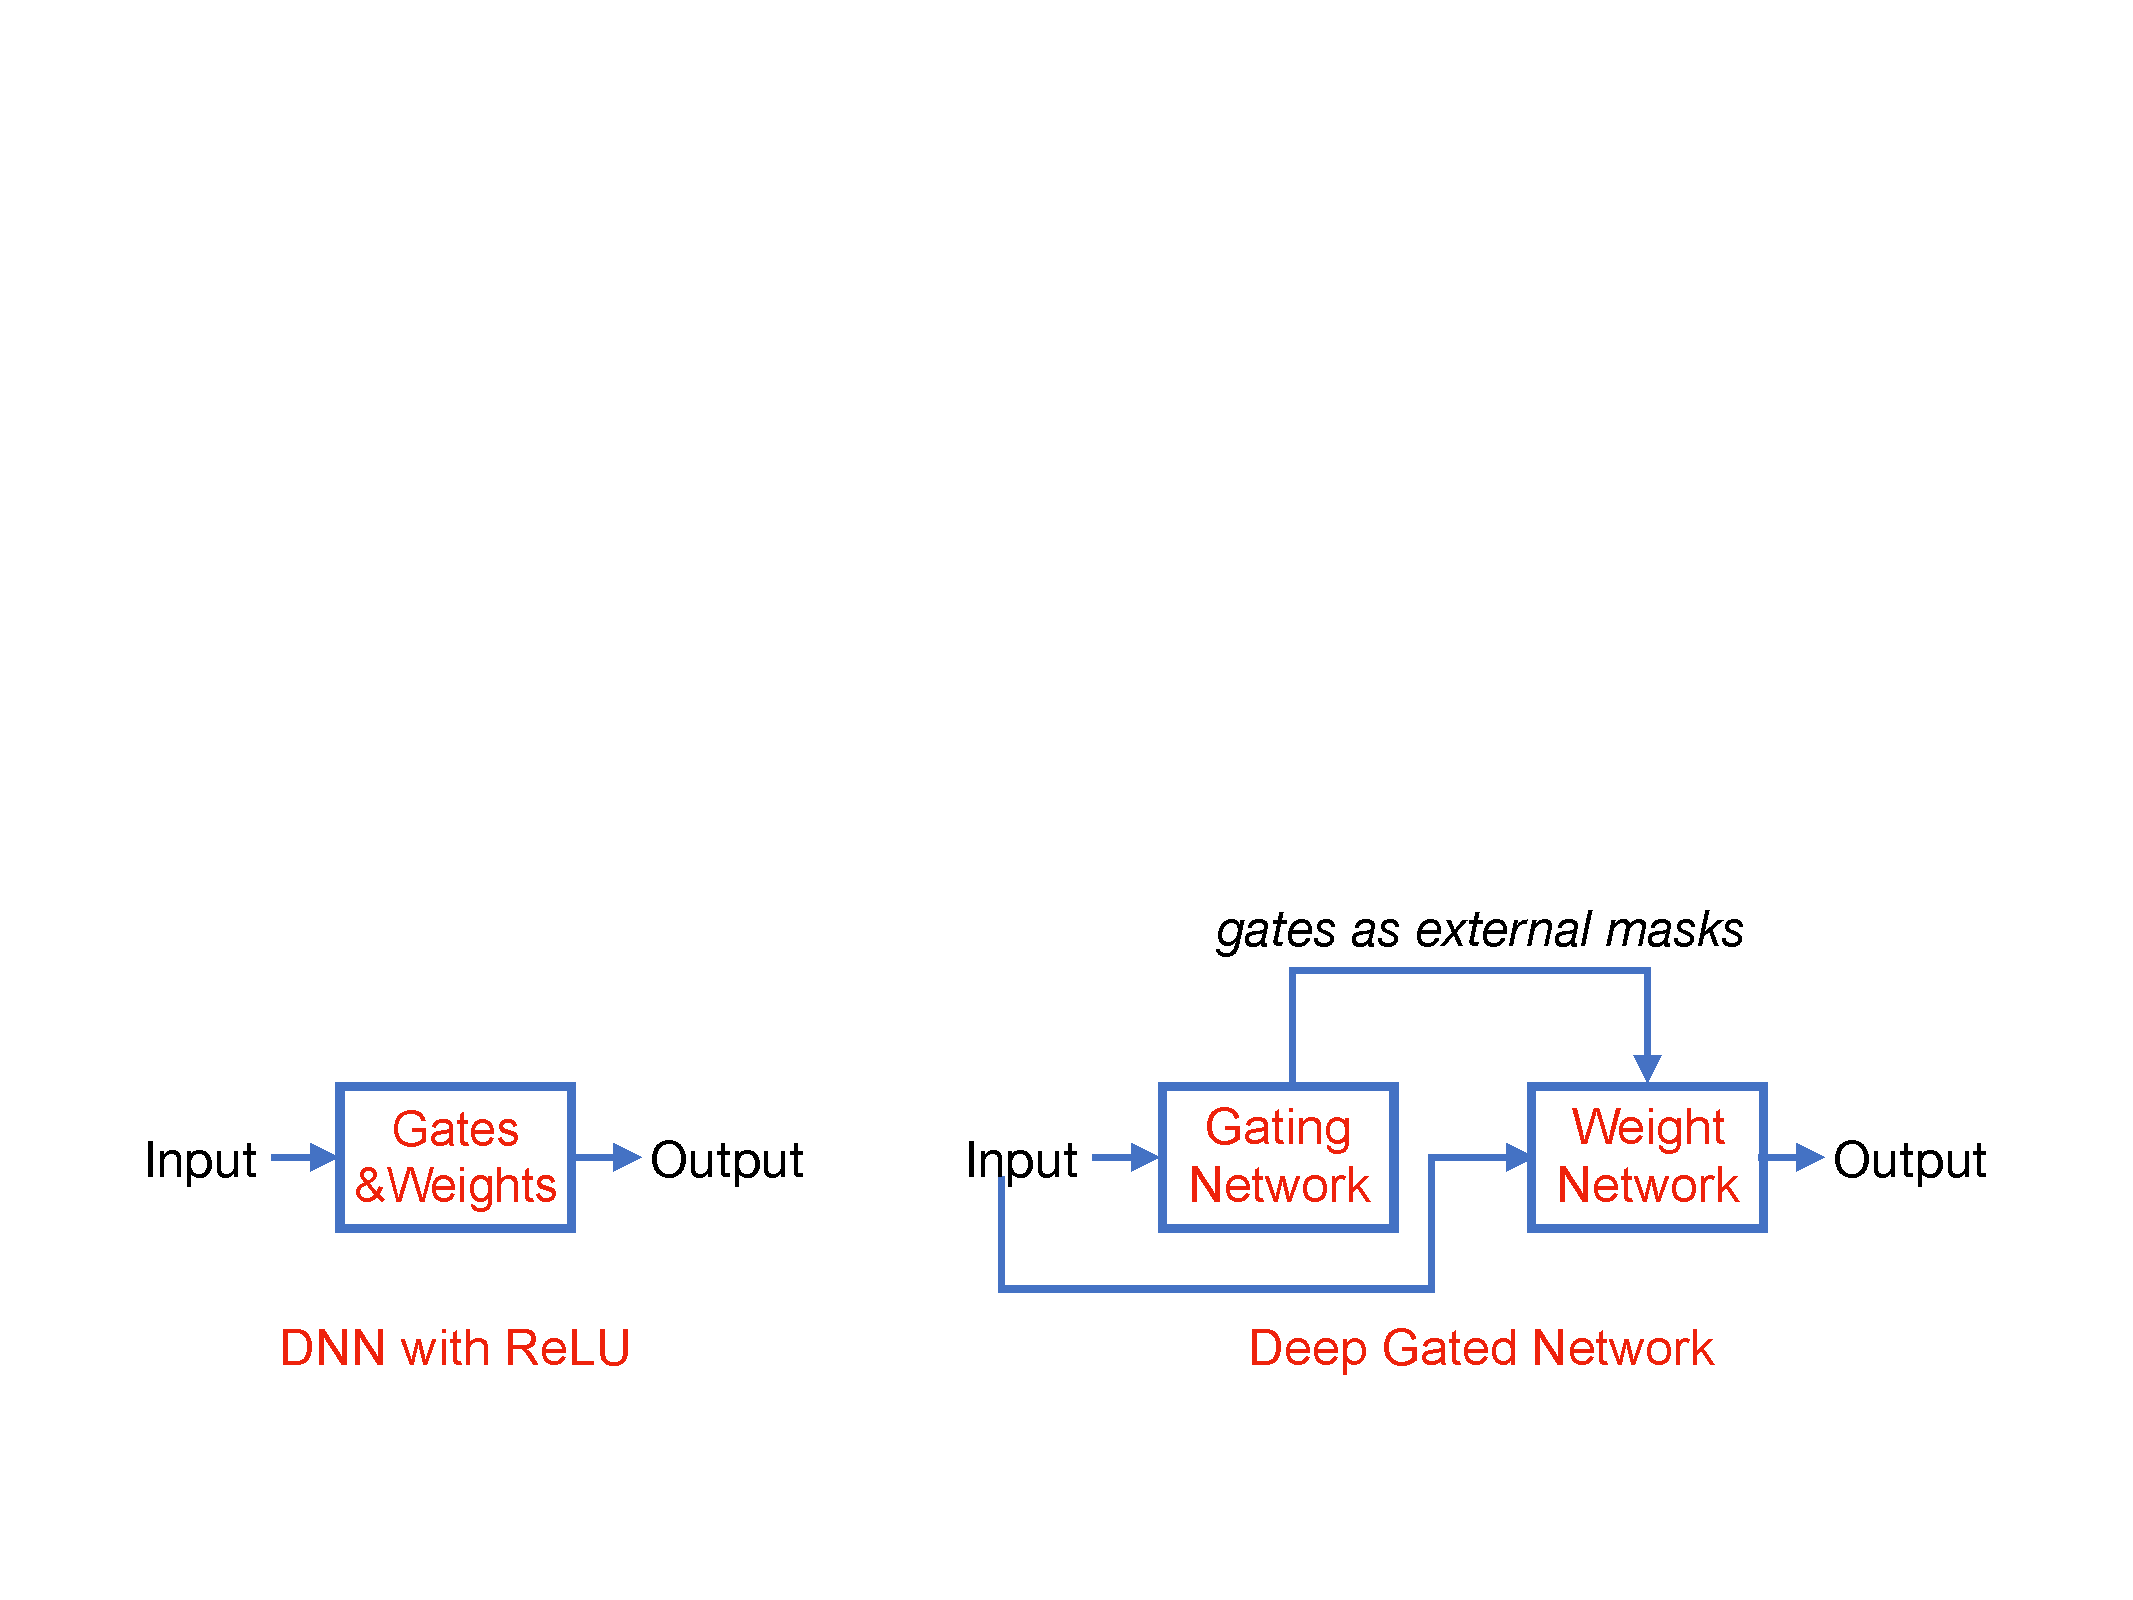
\includegraphics[scale=0.25]{figs/dnn-dgn.pdf}
}
\caption{DNN vs DGN.}
\label{fig:dgn}
\end{figure}
$1.$ \emph{Most information is in the gates:} By using just the gates of a pre-trained DNN (by letting it to be the gating network), the weight network can be trained to match the test performance (within $1\%$ ) of the DNN.

$2.$ \emph{Learning in gates} is the difference between finite width DNN and the infinite width NTK.  

\textbf{Duality simplifies NTK:} \citet{npk} showed that in a DGN, $\text{NTK}=\text{NTK}^{\text{fixed-gate}}+\text{NTK}^{\text{gate-learn}}$, where $\text{NTK}^{\text{fixed-gate}}$ is the kernel corresponding to learning of the weights with the gates fixed and $\text{NTK}^{\text{gate-learn}}$ is the kernel corresponding to learning of gates themselves. Further, $\text{NTK}^{\text{fixed-gate}}$ simplifies into a \emph{neural path kernel} (NPK), a kernel which is solely dependent on the information stored in the gates.

\textbf{NPK Interpretability:} Each input has a corresponding \emph{active sub-network} comprising of the gates that are \emph{on} and weights through such gate. This active sub-network is responsible for producing the output. NPK is a \emph{Hadamard product} of the input Gram matrix and correlation matrix that measures the amount overlap in the active sub-networks for the various pairs input examples. In contrast to the hidden layer outputs, these active sub-networks are physically interpretable as connections.


\textbf{Duality+ NTK:} The overall picture of duality together with NTK can be summarised as follows: (i) training and generalisation of infinite width DNNs is explain by the NTK \citet{arora2019exact,cao2019generalization}, (ii) \citet{npk} showed that most information is in the gates which is characterised by the NPK, (iii) ReLU activation has a special role, i.e., they are gates, (iv) the primary role of the weights is to trigger the ReLU on/off.
\end{comment}
\subsection{Our Contribution: Simplify NPK into atomic units}
\FloatBarrier
\begin{figure}[h]
\centering
\resizebox{\columnwidth}{!}{
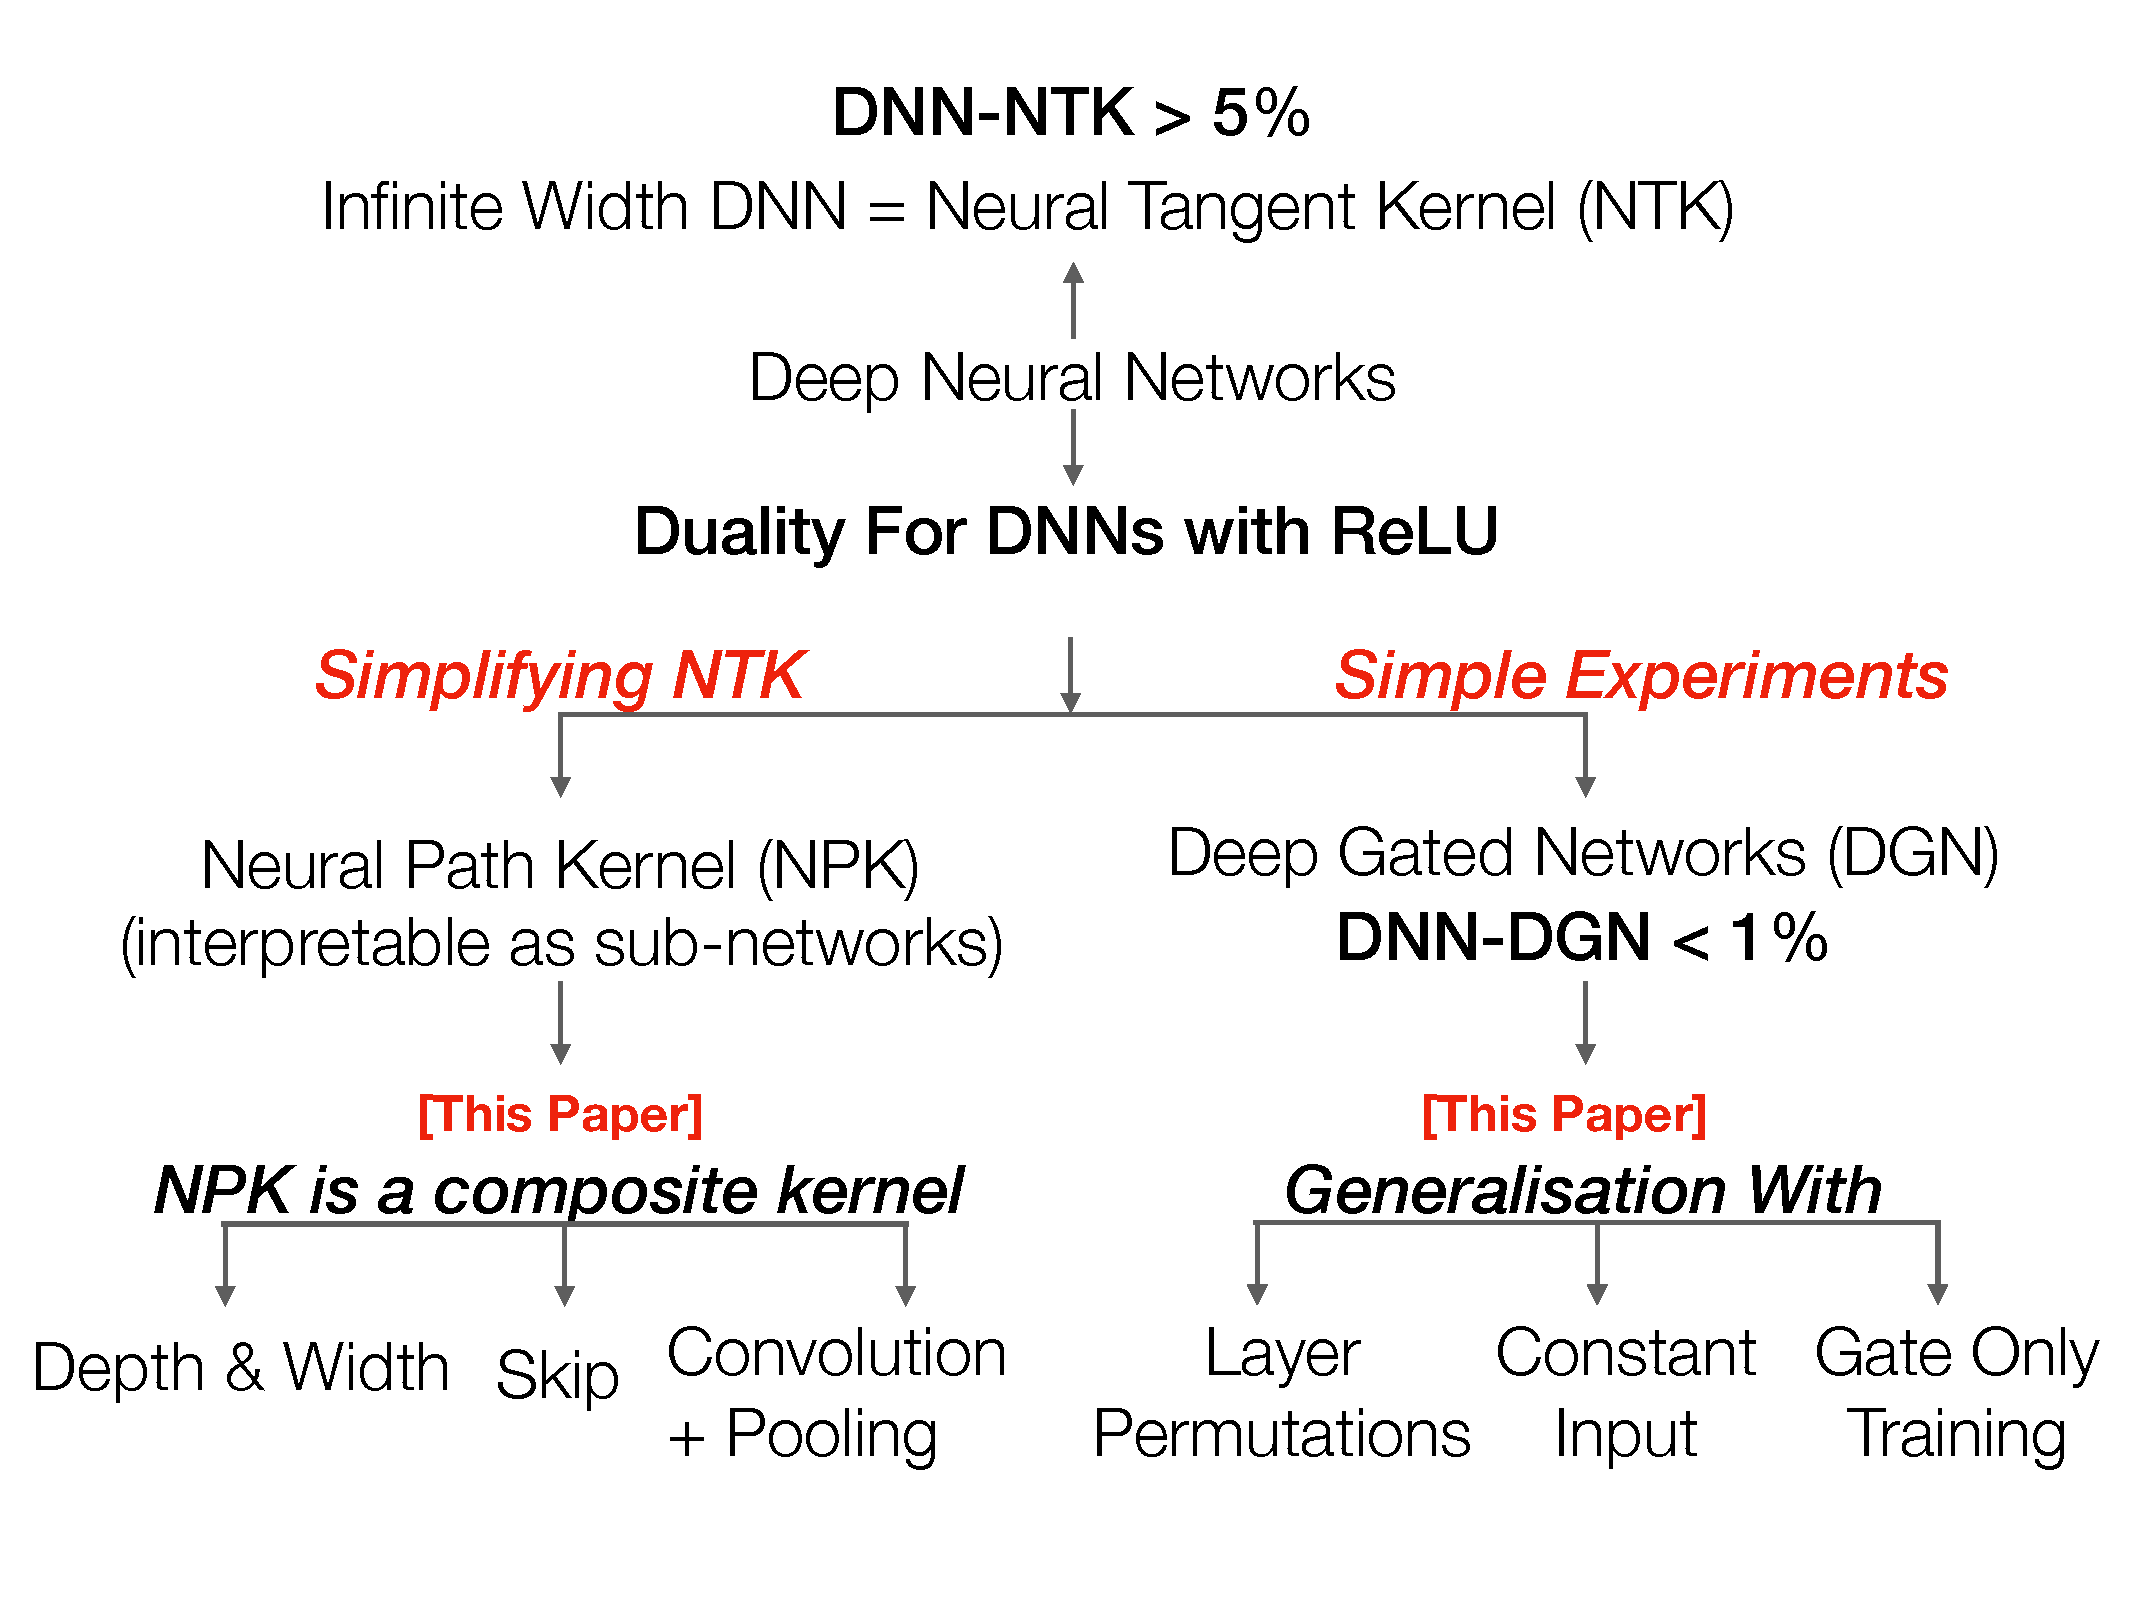
\includegraphics[scale=0.25]{figs/related.pdf}
}
\caption{This paper in relation to (i) NTK, (ii) Duality.}
\label{fig:related}
\end{figure}

 In this paper, we simplify the NPK into \emph{atomic} units to explain roles of width, depth, skip connections and convolutions with pooling. Our novel contributions are as under.

\begin{comment}
\begin{table}
\centering
\begin{tabular}{p{1.75cm}p{2.25cm}p{2.25cm}p{0.01cm}}z
	     &\centering{Primal} 	& \centering{Dual+NTK}&\\\hline
Train, Gen. &\centering\ding{53}    & \centering{\ding{51}}& \\\hline
ReLU          &\centering{\ding{51}: yet another non-linearity} & \centering{\ding{51}: gates that are learnt}&\\\hline
Weights          &\centering{\ding{51}: linear part of a layer} & \centering{\ding{51}: triggers the gates}&\\\hline

\end{tabular}
\end{table}
\end{comment}


\begin{comment}
\begin{table}
\begin{tabular}{ccccccccc}\hline
Primal & A & B & C& D & E& F & G & H\\ \hline
Primal & \ding{53} & \ding{53} & C & D & E& F & G & H\\ \hline
Kernel & A & B & C& D & E& F & G & H\\ \hline
Dual+NTK [This paper]& A & B & C& D & E& F & G & H\\ \hline
\end{tabular}
\end{table}
\end{comment}

$\bullet$ \textbf{Simplifying the NPK:} In fully connected DNNs, we show that (for inputs $x,x'\in\R^{\din}$) NPK$(x,x')=\langle x,x'\rangle\cdot \Pi_{l=1}^{d-1} \frac{H^{\text{lyr}}_l(x,x')}{w}$. Here the most basic atomic units are the gates; stacking ReLUs widthwise in a layer gives rise to a base kernel $\frac{H^{\text{lyr}}_l(x,x')}{w}$ which measures the \emph{average} number of triggered ReLUs for both $x$ and $x'$; stacking layers depth-wise gives rise to the \emph{product} of base kernels. This explains the roles of \emph{width and depth}.

$\bullet$ \textbf{Residual Networks (ResNets)} with skip connections give rise to NPK with a \emph{ sum of product of base kernels}.

$\bullet$ \textbf{Convolutional layers with pooling} renders the NPK \emph{rotationally invariant}. 

$\bullet$ \textbf{Invariances (\Cref{fig:permutations}):} We experimentally verify that DGN performance is invariant to (i) layer permutations ($\Pi_{l=1}^{d-1} \frac{H^{\text{lyr}}_l}{w}$ does not change) and (ii) input tensor with entries equal to $1$ (here, NPK$(x,x')= \text{constant}\cdot \Pi_{l=1}^{d-1} \frac{H^{\text{lyr}}_l}{w}$ depends on the input via the product of the base kernels). This further supports the claim that \emph{most information is in the gates}. %This result shows that standard view that \emph{hidden layer outputs is a red-herring} and the actual feature learning happens in the gates.
\FloatBarrier
\begin{figure}[h]
\centering
\resizebox{\columnwidth}{!}{
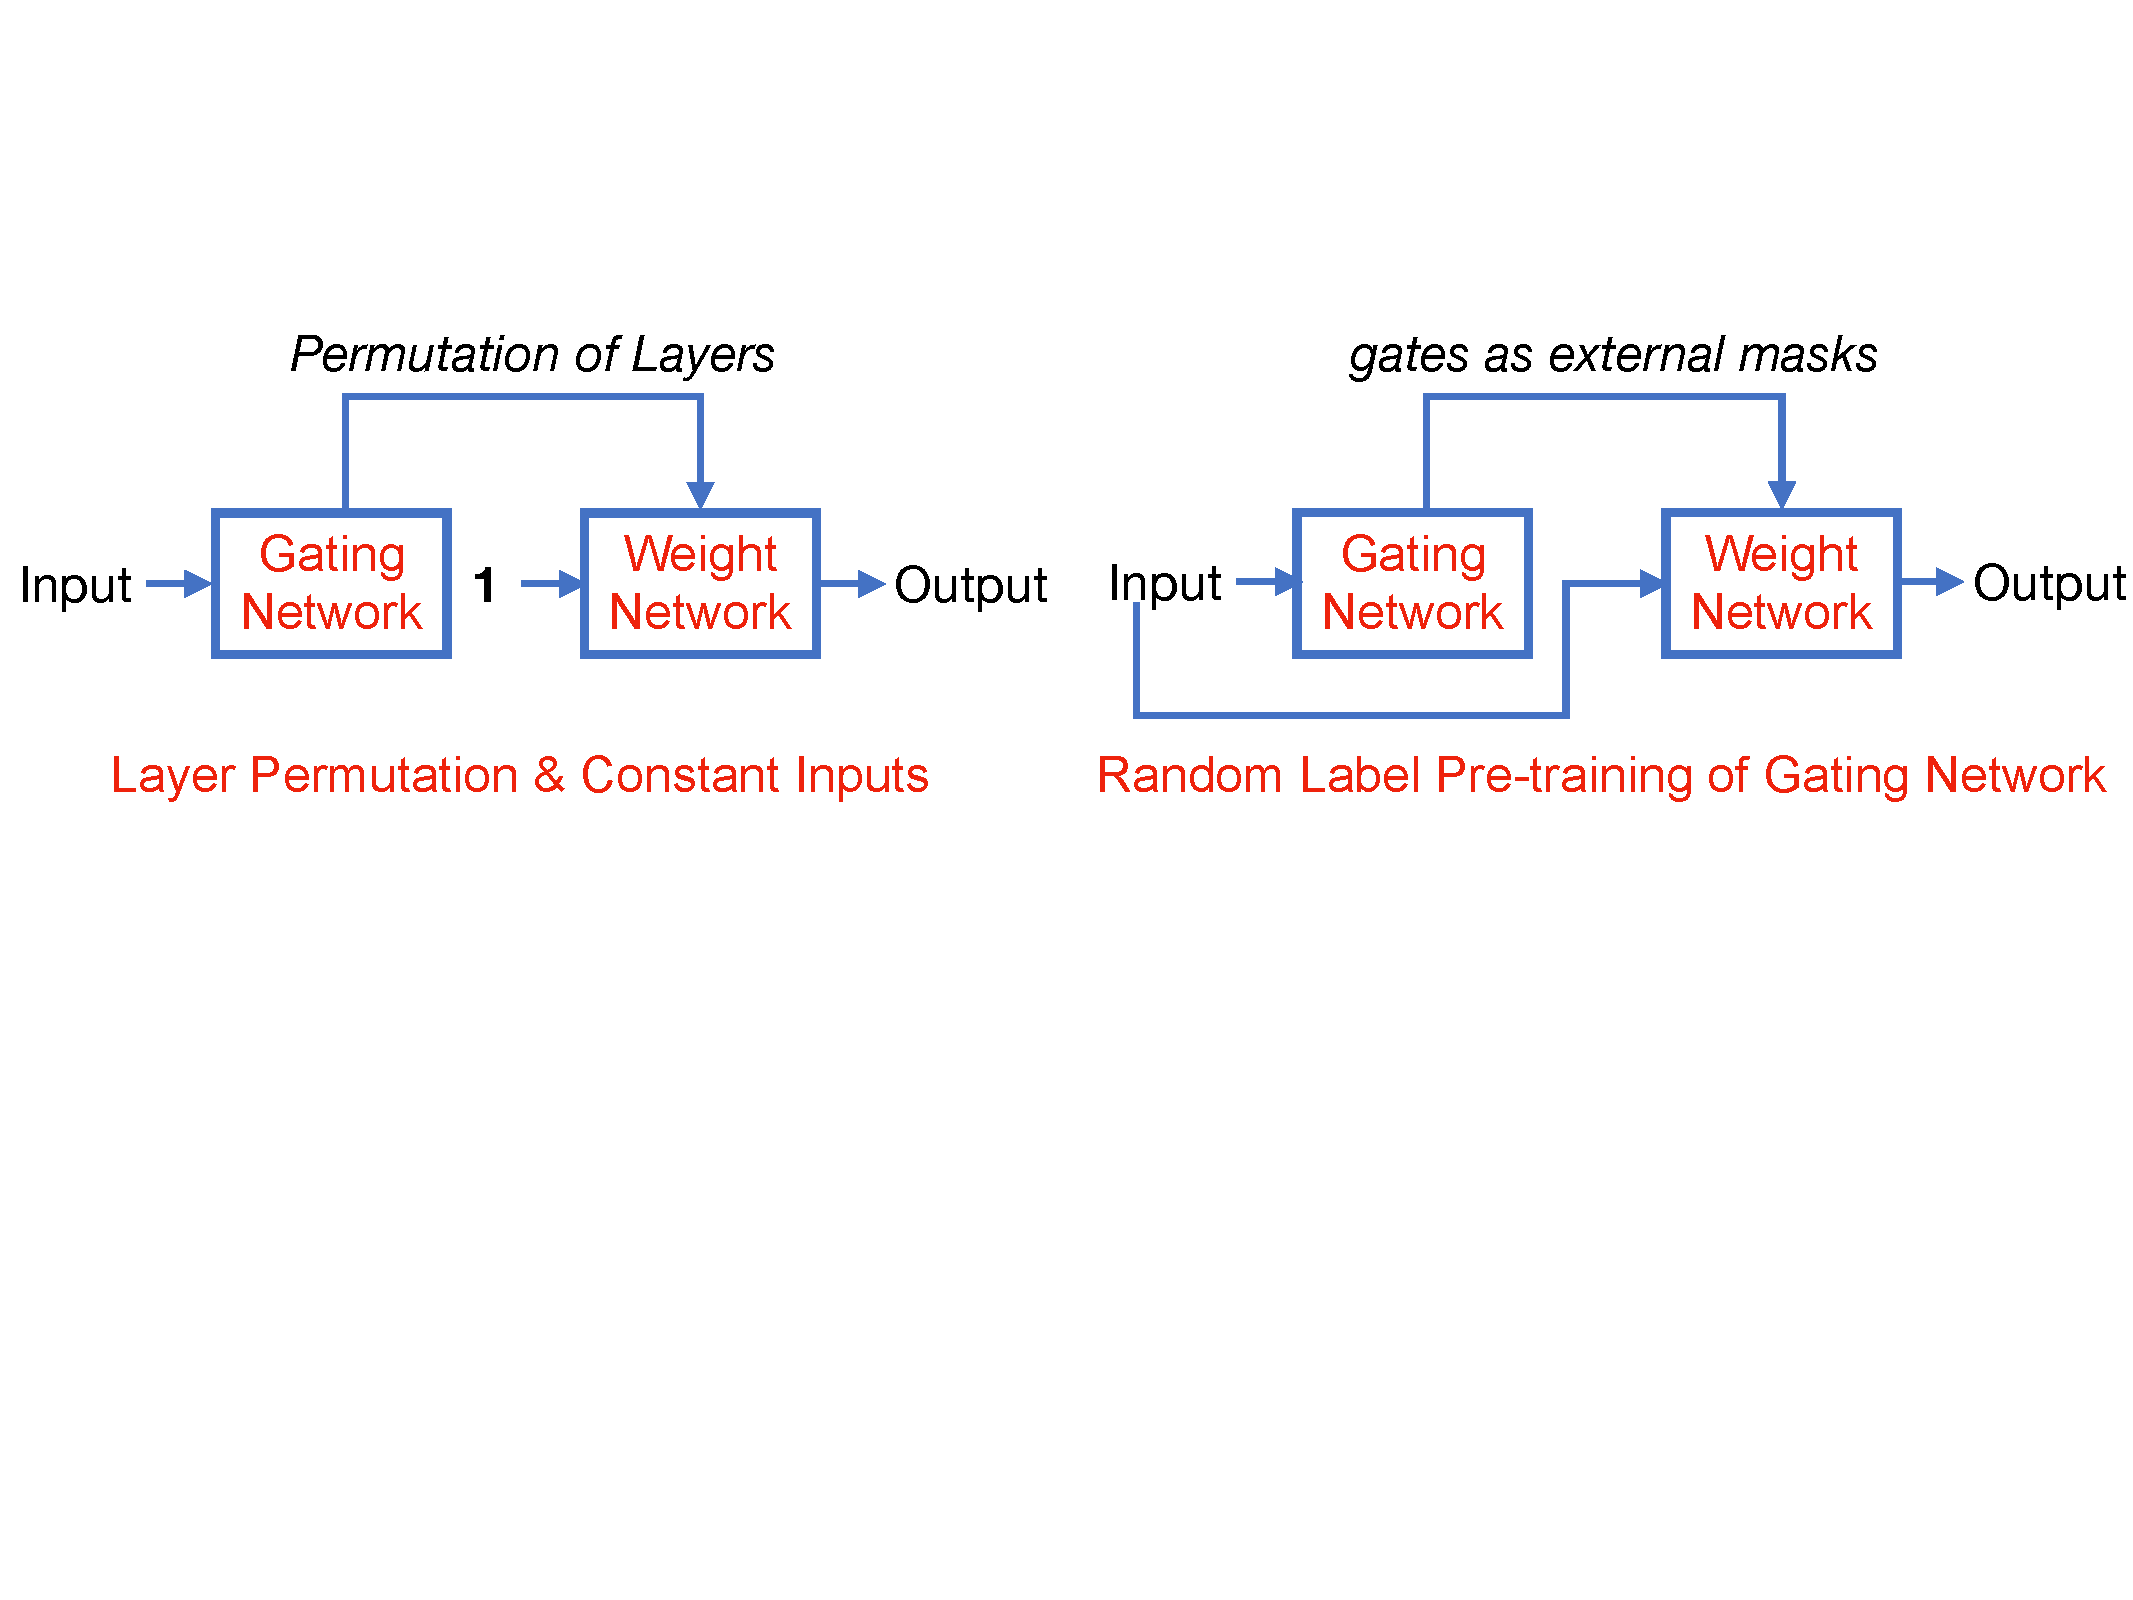
\includegraphics[scale=0.25]{figs/permute.pdf}
}
\caption{Experiments to show that most learning is in the gates.}
\label{fig:permutations}
\end{figure}

$\bullet$ \textbf{Training only the gates} (\Cref{fig:permutations}) on CIFAR-10 achieves a test accuracy of $65\%$.

\textbf{Significance of Duality:} The primal \emph{layer-by-layer} and the dual \emph{path-by-path} views of computations complement each other. The primal view is used in \emph{actual} training via backpropagation and the dual view serves as pedagogical nugget to atomise and interpret DNNs. In particular,\\
$\bullet$ The experimental result on DGN invariance to layer permutation suggests that visually interpreting the hidden layer outputs may not be meaningful. This also tips the balance in favour of the view that gates hold the true features.\\
$\bullet$ Arbitrary gates (not just random) can be examined. Just as a single perceptron is characterised by a hyperplane, a DNN (with ReLU) being a multi-layered-perceptron is \emph{almost completely} characterised by the collection of hyperplanes (associated with the ReLUs that form the DNN).
\begin{table}[h]
\resizebox{\columnwidth}{!}{
\begin{tabular}{|p{1.75cm}|p{3.25cm}|p{2.75cm}|}\hline
	&{Primal} & {Dual + NTK}\\\hline
Output  &layer by layer & path by path \\		\hline
Features & hidden layer output &  gates; ${\color{red}\bm{\dagger}}$layers can be permuted\\\hline
Interpretation  & difficult & sub-network \\\hline
ReLU        &yet another non-linearity & gating property; gates are learnt; \\\hline
Weights     &linear part of a layer & hyperplane related to gates\\\hline
Width         & dimension of features in hidden layer&${\color{red}\bm{\dagger}}$ averaging in base kernels.\\\hline
Depth       &nesting of non-linearity &  ${\color{red}\bm{\dagger}}$ product of base kernels.\\\hline
Skip          & residual error propagation & ${\color{red}\bm{\dagger}}$ sum of product of base kernels.\\\hline
Convolution + Pooling & rotational invariance of features in hidden layer  & ${\color{red}\bm{\dagger}}$ rotational invariance of NPK.\\\hline

\end{tabular}
}
\caption{Primal-Dual Viewpoints. ${\color{red}\bm{\dagger}}=$ novelties in this paper.}
\label{tb:primal-dual}
\end{table}

\begin{comment}
\FloatBarrier
\begin{table}[h]
\centering
\begin{tabular}{p{1.75cm}p{0.75cm}p{0.75cm}p{4cm}p{0.01cm}}
	     &\centering{Primal} &\centering NTK	& \centering{Dual+NTK [This Paper]}&\\
Train + Test &\centering\ding{53}  & \centering{\ding{51}},$*$  & \centering{\ding{51}},$**$& \\
ReLU          &\centering{\ding{53}} & \centering{\ding{53}} & \centering{\ding{51}}&\\
Weights          &\centering{\ding{53}} & \centering{\ding{53}}& \centering{\ding{51}}&\\
Width          &\centering{\ding{53}} & \centering{\ding{53}}& \centering{\ding{51}}&\\
Depth          &\centering{\ding{53}} & \centering{\ding{53}}& \centering{\ding{51}}&\\
Skip          &\centering{\ding{51}} & \centering{\ding{53}}& \centering{\ding{51}}&\\
Conv.+Pool          &\centering{\ding{51}} & \centering{\ding{53}}& \centering{\ding{51}}&\\
\end{tabular}
\caption{Primal-Dual Philosophy.}
\label{tb:primal-dual}
\end{table}
\end{comment}
\begin{comment}
 We consider deep neural networks (DNNs) with \emph{rectified linear units} (ReLUs). For such DNNs, we propose a \emph{pedagogical nugget} ``simple theorems, simple experiments" \citet{Aliresponse} by combining \emph{neural tangent kernel} (NTK) and \emph{dual view}. Our aim is to explain training, generalisation, roles of weights/activation/width/depth/convolutions with pooling/skip connections. Training and generalisation of infinite width DNN 


In this paper, we make two major contributions using the lens of dual view. Firstly, we show that the NPK has a \emph{compositional} structure. The results are listed below.

$\bullet$ \emph{Fully Connected DNN (FC-DNN):} In this case, the NPK involves a \emph{ Hadamard product of base kernels} structure. Here the most basic unit is the gate.  stacking ReLUs widthwise in a layer gives rise to a base kernel which measures the \emph{average} number of triggered ReLUs; stacking layers depthwise gives rise to a \emph{Hadamard product}. This result also explains the roles of \emph{width and depth}.

$\bullet$ \emph{Residual networks with skip connections:} In this case, the NPK involves a  \emph{ sum of Hadamard product of base kernels} structure.

$\bullet$ \emph{Convolutional layers with pooling:} In this case, the NPK  has a  \emph{rotational invariant} structure.

Our second major contribution is an ablation study to argue that the standard view that hidden layer outputs is a red-herring and the actual feature learning happens in the gates. To bolster our case, we build combinatorially many models by,

1. permuting the order of the layers when we apply them as external masks,

2. providing a tensor with all entries $1$ instead of the input image. 

We observe in our experiments that the performance is robust to such combinatorial variations.

We also show experimentally how training with random labels affects the gates, and experimentally verify how skip connections improve the conditioning of the underlying NTK.
\end{comment}
\subsection{Organisation and Notation}
\Cref{sec:ntk,sec:dual,sec:dgn} contains brief overview of the NTK, duality and the DGN setup. \Cref{sec:fc} contains the result which explains the role of activations, weights, depth and width. \Cref{sec:res,sec:conv} contain the result that explains the role of skip connections and convolutions with pooling respectively. \Cref{sec:exp} contains the numerical experiments.

We denote the set $\{1,\ldots, n\}$ by $[n]$. For $x,y\in\R^m$, $\ip{x,y}=x^\top y$. The dataset is denoted by $(x_s,y_s)_{s=1}^n\in\R^{\din}\times \R$. For an input $x\in\R^{\din}$, the output of the DNN  is denoted by $\hat{y}_{\Theta}(x)\in\R$, where $\Theta\in\R^{\dnet}$ are the collection of all weights. $\nabla_{\Theta}(\cdot)$ denotes the gradient of $(\cdot)$ with respect to $\Theta$. 